\chapter{Shluková analýza} \label{sec:clusteranalysis}
Shluková analýza je možná jeden z nevíce zkoumaných problémů v oblasti strojového učení a dolování dat~\cite{Aggarwal13}. Lze ji využít ve velkém množství oborů a disciplín jako například sumarizace a segmentace dat, cílený marketing a nebo již zmíněné strojové učení~\cite{Jain10, Kaufman90}. Základní problém shlukování se dá formulovat následovně: \textit{Máme množinu vstupních bodů, snažíme se je rozdělit tak, aby skupiny obsahovaly co nejpodobnější body.} Tato definice je velmi vágní, protože se různé definice problému velice liší v závislosti na specifických vlastnostech použitých modelů dat~\cite{Aggarwal13}. Pokud uvážíme například generační model dat, budeme pravděpodobně využívat podobnost založenou na genetických mechanismech, kdežto podobnost založenou na vzdálenosti budeme používat především u obecných modelů založených na číslech. Velký vliv na definici shlukové analýzy mají také vlastnosti vstupních dat.


%The problem of the cluster analysis is perhaps one of the most widely studied problems in machine learning or data mining~\cite{Aggarwal13}. It has numerous application in disciplines such as machine learning, summarization, segmentation, and target marketing~\cite{Jain10, Kaufman90}.
%The basic problem of clustering may be stated as follows:\textit{Given a set of data points, find groups in data so each group consist of as similar points as possible.} This definition is very rough, because the variations in the problem definition can be significant, depending upon the specific data model used~\cite{Aggarwal13}. For example, a generative model may define similarity on the basis of probabilistic generative mechanism, whereas a distance-based approach will use a traditional distance function for the quantification. Also the data properties has a significant impact on the definition.
%In this context, objects are similar when their properties has same values or differs minimally in comparison to same property of other nearest objects or all objects in cluster. This means that each cluster contains objects that are more similar to nearest neighbors or all objects from cluster than objects from other clusters. Hence the cluster analysis may be performed only on sets of objects which must be to each other comparable - we must be able.to decide how much are two objects similar. This analysis has a wide range of applications, such as data mining, pattern recognition or machine learning.\\
\section{Definice}
Vzhledem k tomu, že shluková analýza je velmi různorodá, zahrnuje mnoho algoritmů, které se mohou značně lišit. Ty závisí na datovém modelu a konkrétní úloze~\cite{Aggarwal13}. Jsou také odlišné v definici shluku a v metodách hledání shluků. Nejčastější definice shluků jsou následující: Shluky jsou skupiny s malou vzdáleností mezi objekty ze stejného shluku, husté oblasti vstupních dat, intervaly nebo jednotlivé statistické distribuce.\\

%Because the cluster analysis is a diverse topic, there are many underlaying algorithms, which could vary greatly. They depend on a data domain and a problem scenario~\cite{Aggarwal13}. They are also different in a cluster definition and in cluster search methods. Cluster most common definitions are following: Clusters are groups with %small distances between the objects from the same cluster, dense areas of the input data, intervals, or each particular statistical distribution.\\
%If we want to define cluster analysis more precisely, it is function $f$ which groups objects $o \in O$, where $O$ is input data set and splits them into subsets. We need also the function $s$ which compares two objects and determines, how much are these objects similar $s: O \times O \to \mathbb{R}$.The task is to split items into subsets so the distances between objects from same subset are minimal. $$min \sum_{c=1}^nO_c:\sum_{i,j=1}^{|O_c|}s(o_i,o_j);o_{i,j}\in O_c;\cap_{c=1}^nO_c=O$$

Samotná shluková analýza by mohla být provedena na mnoha typech dat, ale v této práci se zaměříme především na vektorové prostory, abychom mohli definovat shlukovou analýzu následujícím způsobem: Vezmeme reálný vektor s dimenzí $d$ jako objekt, kde každý prvek vektoru představuje vlastnost objektu. Množina vektorů $V$ nad polem $F$ musí splňovat axiomy vektorového prostoru s operacemi $\oplus: V \times V \to V$ zvané sčítání a $\otimes:F \times V \to V$ zvané násobení:
%Cluster analysis itself could be performed on many types of data but in this thesis, we will focus mainly on vector spaces so we could define the cluster analysis in following way:
%We will take a real vector with dimension $d$ as an object, where each element of vector presents an object property. The set of vectors $V$ over field $F$ must fulfill axioms of the vector space with operations $\oplus: V \times V \to V$ called addition and $\otimes:F \times V \to V$ called multiplication:
\begin{enumerate}
\item $(\forall \vec{u}, \vec{v} \in V):\vec{u} \oplus \vec{v} = \vec{v} \oplus \vec{u}$ \textit{(komutativita pro sčítání vektorů)}
\item $(\forall \vec{u}, \vec{v}, \vec{w} \in V):(\vec{u} \oplus \vec{v}) \oplus \vec{w} = \vec{u} \oplus (\vec{v} \oplus \vec{w})$ \textit{(asociativita pro sčítání vektorů)}
\item $(\exists \vec{0})(\forall \vec{v} \in V):\vec{v} \oplus \vec{0} = \vec{v}$ \textit{(existence nulového vektoru)}
\item $(\forall \vec{u} \in V)(\exists \vec{v} \in V):\vec{u} \oplus \vec{v} = \vec{0}$ \textit{(existence opačného vektoru)}
\item $(\forall a,b \in F)(\forall \vec{v} \in V):(a \otimes b) \otimes \vec{v} = a \otimes (b \otimes \vec{v})$ \textit{(asociativita pro násobení vektoru)}
\item $(\exists \textbf{1} \in F)(\forall \vec{v} \in V):\textbf{1} \otimes \vec{v} = \vec{v}$ \textit{(invariance vektoru při vynásobení jednotkovým prvkem tělesa)}
\item $(\forall a,b \in F)(\forall \vec{v} \in V):(a + b) \otimes \vec{v} = (a \otimes \vec{v}) \oplus (b \otimes \vec{v})$ \textit{(distributivita násobení vektoru vzhledem ke sčítání prvků tělesa)}
\item $(\forall a \in F)(\forall \vec{u}, \vec{v} \in V):a \otimes (\vec{u} \oplus \vec{v}) = (a \otimes \vec{u}) \oplus (a \otimes \vec{v})$ \textit{(distributivita násobení vektoru vzhledem ke sčítání vektorů)}
\end{enumerate}

Také musíme mít metrickou funkci $d:V \times V \to F$ která splňuje axiomy metriky:\\ \\
$ \forall  u, v, w \in V$
\begin{enumerate}
\item $d(u, v)\geq 0$ \textit{(nezápornost)}
\item $d(u, v) = 0 \iff u = v$ \textit{(identita)}
\item $d(u, v) = d(v, u)$ \textit{(symetrie)}
\item$d(u, v) \leq d(u, w) + d(w, v)$ \textit{(trojúhelníková nerovnost)}
\end{enumerate}

Hlavní úkol je stejný jako ve obecné definici. Musíme najít systém podmnožin tak, aby vzdálenosti mezi vektory v jedné podmnožině byly minimální.
%The main task is same as in common definition. We need to find a system of subsets so the distances between vectors in one subset is minimal.

\subsection{Vzdálenosti}
Jak jsme se zmínili na začátku této části, shluková analýza by mohla být provedena na mnoha typech dat. Tato různorodost se odráží v širokém rozsahu použitelných funkcí pro výpočet vzdálenosti (nebo podobnosti), protože konkrétní typ dat vyžaduje specifickou metriku. Vzdálenost je pro shlukovou analýzu velmi důležitá, protože často určuje, zda je shluková analýza použitelná na konkrétní typ dat. Jelikož v této práci se budeme věnovat především vektorovým prostorům, začneme s obecnou normovanou vzdáleností použitelnou v tomto prostoru: $$\|a-b\|_p=\sqrt[\leftroot{-1}\uproot{3}\scriptstyle p]{\sum_i |a_i - b_i|^p} $$
Nejčastěji používaná vzdálenost $L_p$ je vzdálenost $L_1$ zvaná \textbf {Manhattanská vzdálenost} nebo $L_2$ vzdálenost zvaná \textbf {Eukleidovská}.
Protože výpočty odmocnin jsou obtížné, mohli bychom zjednodušit vzdálenost tím, že vynecháme výpočet odmocnin. Toto neporušuje metrické axiomy a obvykle se nazývá \textbf {čtvercová eukleidovská vzdálenost}.\\

%Because all of these algorithms counts distance, appropriate metric must be used.
%\begin{description}
%\item[Manhattan distance $L_1$] $$\|a-b\|_1=\sum_i |a_i - b_i| $$
%\item[Euclidian distance $L_2$] $$\|a-b\|_2=\sqrt{\sum_i (a_i - b_i)^2 }$$
%\item[Squared Euclidian distance $L_2^2$] $$\|a-b\|_2^2=\sum_i (a_i - b_i)^2 $$
%\item[$p$-norm distance $L_p$] $$\|a-b\|_p=\Big(\sum_i |a_i - b_i|^p\Big)^\frac{1}{p} $$
%\item[Maximum distance $L_\infty$] $$\|a-b\|_\infty=\lim_{p\to\infty}\Big(\sum_i |a_i - b_i|^p\Big)^\frac{1}{p}=\max_i |a_i - b_i| $$
%\end{description}
U dalších datových typů dat uvádíme několik příkladů nevektorových prostorů. Můžeme například použít vzdálenost použitelnou ve statistice, jako je \textbf{Mahalanobisova vzdálenost} a \textbf{Wassersteinova metrika}

\subsubsection{Mahalanobisova vzdálenost}
Je užitečná, pokud potřebujeme vypočítat vzdálenosti mezi bodem $ P$ a distribucí $D$. Hlavní myšlenka této vzdálenosti je měření odlišnosti $P$ od průměru $D$.
Pokud máme pozorování $p = (p_1,..., p_n)^T$ a střední hodnotu pozorování $\mu=(\mu_1,...,\mu_n)^T $ a matici kovariance $S$, Mahalanobisova vzdálenost je definována jako:
%Is useful if we need to compute distances between a point $P$ and distribution $D$. The main idea of this distance is measuring ho differs $P$ from the mean of $D$.
%If we have observation $p=(p_1,...,p_n)^T$ a mean of set of observations $\mu=(\mu_1,...,\mu_n)^T$ and a covariance matrix $S$, the Mahalanobis distance is defined as:
$$D_M(x) = \sqrt{(x - \mu)^T S^{-1} (x-\mu)}$$

\subsubsection{Wassersteinova metrika}
Další vzdálenost použitá ve statistice je Wassersteinova metrika (nazývaná též Earth mover's distance (EMD))~\cite{Vallender73}. Tato metrika se používá pro výpočet vzdálenosti mezi dvěma pravděpodobnostními distribucemi na daném metrickém prostoru $M$. Existuje analogie s posouváním "zeminy" nahromaděné stejným způsobem jako tvar distribuce pravděpodobnosti. Vzdálenost je množství "zeminy", která musí být přemístěno tak, aby se změnil tvar hromady na jiný tvar určený rozložením druhé pravděpodobnosti. Množství je pak ještě potřeba vynásobit vzdáleností, o kterou je třeba zeminu přesunout. Tato vzdálenost je definována takto: \\
Nechť $X$ je metrický prostor s metrikou $\ rho$ a $\mathfrak {B}$ je $\ sigma$-algebra Borelovských podmnožin $X$. Wassersteinova vzdálenost $R(P, Q)$ mezi rozdělení pravděpodobnosti $P$ a $Q$ na $(X, \mathfrak{B}) $ je definována jako:
%Another distance used in statistics is Wasserstein metric (also called Earth mover's distance (EMD))~\cite{Vallender73}. This metric is used for compute distance between two probability distributions on given metric space $M$. There is analogy with moving ``earth'' piled up in same way as shape of probability distribution. The distance is amount of ``earth'' which must be moved to change the shape of pile into another shape specified by second probability distribution times the distance it has to be moved. This distance is defined by following way:\\
%Let $X$ be a metric space with metrix $\rho$ and $\mathfrak{B}$ be the $\sigma$-algebra of Borel subsets of $X$. The Wasserstein distance $R(P,Q)$ between probability distributions $P$ and $Q$ on $(X, \mathfrak{B})$ is defined as:
$$R(P,Q)=\inf\mathbf{E}\rho(\xi, \sigma)$$
kde $\inf$ se bere  ze všech možných dvojic náhodných proměnných $\xi$ a $\sigma$ s distribucí $P$ a $Q$.\\

Existují také prostory, které nemají s matematikou mnoho společného, ale obsahují objekty, které jsou porovnatelné.
%There are also spaces, which are even not from mathematics but which contains objects that are also comparable.

\subsubsection{Levenshteinova vzdálenost} Levenshtein distance is used for edit distance between two strings $a, b$ and it is recursively defined by following definition:
\begin{equation*}
lev_{a,b}(i,j)=
\begin{cases}
max(i,j) & $if $ min(i,j)=0, \cr
min \begin{cases}
lev_{a,b}(i-1,j) + 1 \cr
lev_{a,b}(i,j-1) + 1 \cr
lev_{a,b}(i-1,j-1) + dif(a_i,b_j)
\end{cases} & $otherwise$
\end{cases}
\end{equation*}
Where \begin{equation*}
dif(a_i,b_j)=
\begin{cases}
0 & $if $ a_i = b_j, \cr
1 & $otherwise$
\end{cases}
\end{equation*}

\subsubsection{Signature Quadratic Form Distance}
Tato metrika je velice užitečnou pro porovnávání multimediálních objektů, které mohou být popsány různými charakteristikami. Problém je v tom, že se tyto charakteristiky mohou lišit ve struktuře a velikosti, takže jsme nemůžeme použít vzdálenosti popsané dříve. Vlastnost každého objektu je popsána vektorem dvojic centroidů z prostoru vlastností $\mathbb{FS}$ a jeho váhy z $\mathbb{R^{+}}$.
Nepočítáme tedy vzdálenosti mezi vlastnostmi, ale právě pomocí Signature Quadratic Form Distance~\cite{Beecks10} a používáme funkce podobnosti.
Matematicky je Signature Quadratic Form Distance (SQFD) definovaná pro dvě sady vlastností $S^{q} = \{\{c_i^q, w_i^q\}|i=1,...,n\}$ and $S^{o} = \{\{c_i^o, w_i^o\}|i=1,...,m\}$ a funkce podobnosti $f_s(c_i, c_j)\to \mathbb{R}$ takto:
$$SQFD_{f_s}(S^q,S^o)=\sqrt{(w_q|-w_o)A_{f_n}(w_q|-w_o)^T}$$
Kde $A_{f_n} \in \mathbb{R}^{(n+m)\times(n+m)}$ je matice podobnosti vygenerovaná aplikací funkce podobnosti $f_s$ na odpovídající centroidy  ($a_{ij}-f_s(c_i,c_j)$) a operátor $|$ znamená zřetězení dvou vektorů, takže $w_q|-w_o = (w_1^q,...,w_n^q,-w_1^o,...,-w_m^o)$\\
%This metric becomes really useful for comparing multimedia objects, which could be described by signatures. Problem is that these signatures could differ in structure and size so we could not use distances described before. The feature of each object is described by a vector of pairs of centroid from feature space $\mathbb{FS}$ and its %weight from $\mathbb{R^{+}}$.
%Than we do not count distances between the feature signatures but in Signature Quadratic Form Distance~\cite{Beecks10}, the similarity functions are used.
%Mathematically, Signature Quadratic Form Distance (SQFD) is defined for two feature signatures $S^{q} = \{\{c_i^q, w_i^q\}|i=1,...,n\}$ and $S^{o} = \{\{c_i^o, w_i^o\}|i=1,...,m\}$ and a similarity function $f_s(c_i,c_j) \to \mathbb{R}$ as:
%$$SQFD_{f_s}(S^q,S^o)=\sqrt{(w_q|-w_o)A_{f_n}(w_q|-w_o)^T}$$
%where $A_{f_n} \in \mathbb{R}^{(n+m)\times(n+m)}$ is the similarity matrix generated by applying similarity function $f_s$ to the corresponding centroids ($a_{ij}-f_s(c_i,c_j)$) and operator $|$ means concatenation of two vectors, so $w_q|-w_o = (w_1^q,...,w_n^q,-w_1^o,...,-w_m^o)$\\

Vzhledem k tomu, že existuje mnoho možností vzdálenostních funkcí pokrývající mnoho datových typů, shluková analýza má velmi široký rozsah použitelnosti a není omezena konkrétními datovými typy. Protože v této diplomové práci jsme nemohli pokrýt všechny tyto možnosti, zaměřili jsme se pouze na vektorové prostory.

\section{Organizace shluků} \label{sec:clusterorganization}
Uspořádání objektů do shluků lze provádět několika způsoby, které závisí na struktuře shluků a počtu shluků, do kterých daný objekt patří.
%Object organization into clusters could be done several ways depends on structure of clusters and number of clusters into which an object belongs.
\begin{description}
\item[Pevné shlukování] je shlukování, kde každý objekt patří k jednomu a jedinému shluku. To znamená, že tvrdá shlukování vytváří systém, kde jsou shluky disjunktní množiny.
\item[Neostré (fuzzy) shlukování] také přiřazuje objekty do shluků, ale rozdíl je, že objekt může patřit více než jednomu shluku. Členství objektu ve shluku je určeno podle úrovně nebo procenta členství, takže objekt může patřit k shluku více či méně na základě podobnosti.
\item[Hierarchické shlukování] je tvořené hierarchicky uspořádanými shluky, které vytváří systém podmnožin. Sjednocení dvou shluků je buď prázdná množina, nebo jeden se z nich. Shluky tedy vytvářejí struktury jako n-ární stromy. Z důvodu složitosti hierarchického shlukování se v této práci zabýváme pouze nehierarchickým typem.
\end{description}
Pro všechny tři typy existuje verze shlukování, která vynechává izolované objekty vzdálené od ostatních. Tyto objekty se nazývají odlehlé hodnoty a jsou ponechány nepřiřazené. Protože výpočet bez přísně přiřazených objektů je složitý a nepřináší mnoho výhod, v této práci jsme se zaměřili pouze na shlukování bez odlehlých hodnot.s\\

Existuje mnoho modelů shluků, ale v další části~\ref{sec:clustermodels} budou popsány pouze ty nejznámější. Jedním z důvodů, proč jich existuje velké množství, je to, že "shluk" nelze přesně definovat~\cite{EstivillCastro02}. Druhým důvodem je široká použitelnost této úlohy, takže lidé z různých oborů se k tomuto problému staví podle toho, jak je v daném oboru shluku chápán.\\
%There are many cluster models but in next section~\ref{sec:clustermodels}, only the best known will be described. One of the reasons why there exists a large amount of them is that the ``cluster'' cannot be precisely defined~\cite{EstivillCastro02}. Second reason is really wide applicability of this task so people from different departments approach this problem differently, because their notion of cluster differs significantly. \\

\section{Shlukové modely a algoritmy} \label{sec:clustermodels}
Existuje mnoho shlukových algoritmů, protože existuje také mnoha shlukových modelům. Problémem ovšem je, že neexistuje univerzální algoritmus, který pokrývá všechny shlukové modely. Všechny algoritmy byly navržen tak, aby pokrývaly jeden model nebo nějakou podmnožinu modelů a obvykle jsou slabé nebo nevhodné pro jiné modely.
%There exist many clustering algorithms because of many cluster models. Problem is that there exist no universal algorithm, such an algorithm that covers all cluster models. Each algorithm was designed to cover one model or a subset of models and usually it is weak or not applicable for other models.

\subsection{Shlukové modely}
Protože neexistuje jednotná definice shluku, existuje také mnoho definice shlukových modelů. V následující části budou popsány nejznámější modely.

\begin{figure}[h]
\centering
\begin{subfigure}{.49\textwidth}
  \centering
  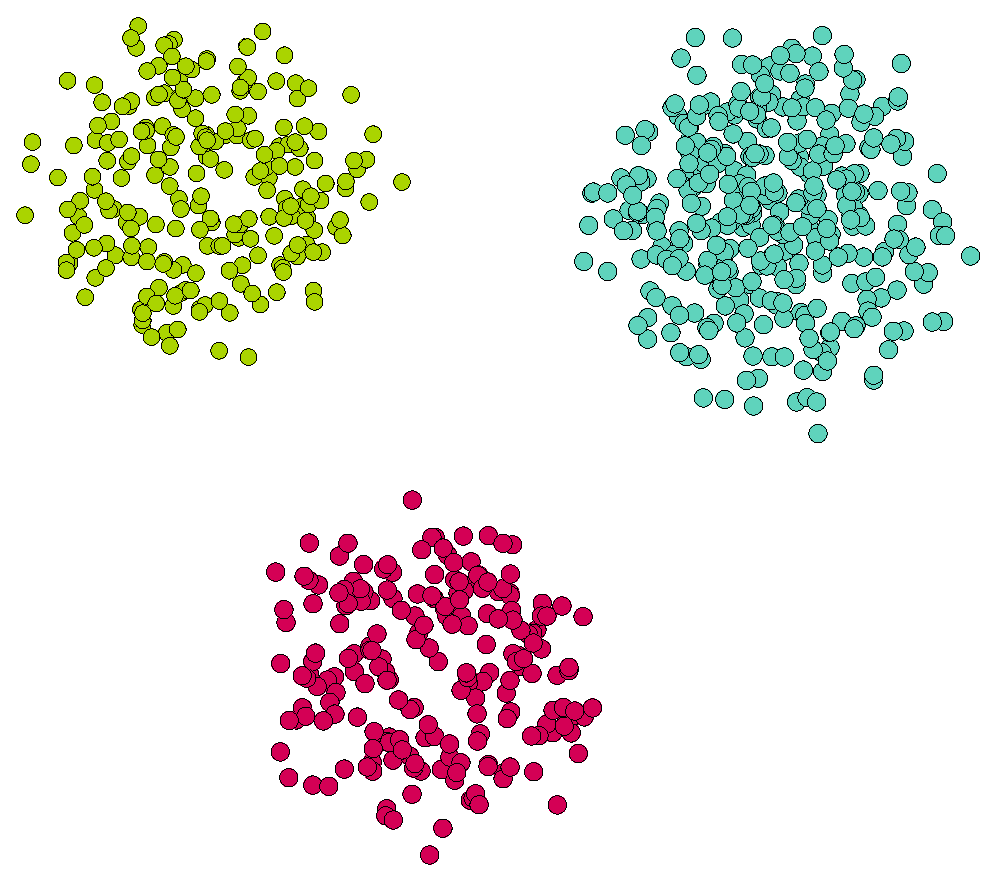
\includegraphics[width=.5\linewidth]{img/wellSeparatedObjects.eps}
  \caption{Dobře oddělené shluky}
  \label{fig:wellSeparatedObjects}
\end{subfigure}
\begin{subfigure}{.49\textwidth}
  \centering
  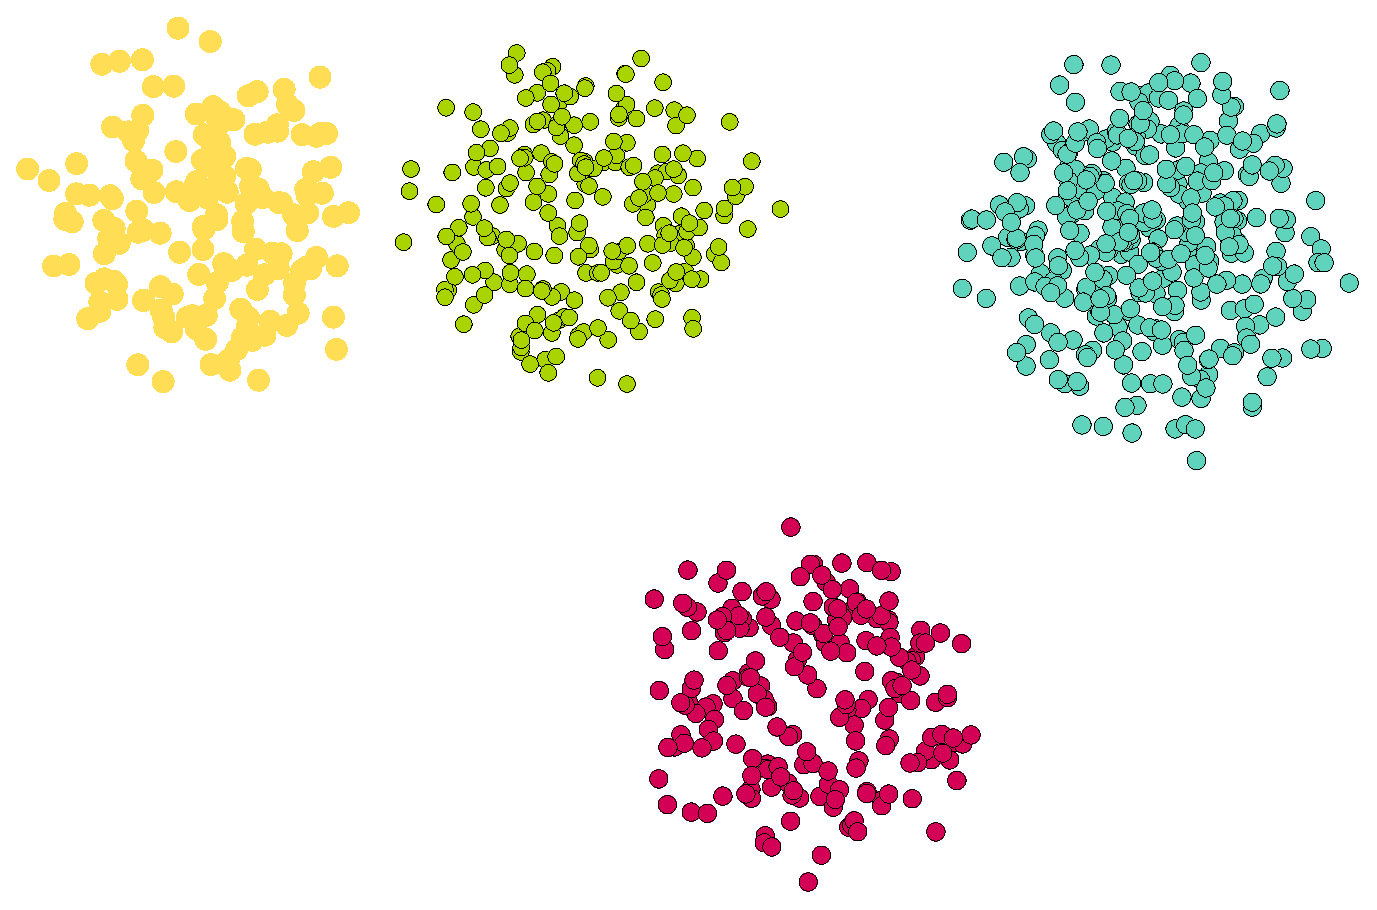
\includegraphics[width=.5\linewidth]{img/centerBasedClusters.eps}
  \caption{Shluky založené na centroidech}
  \label{fig:centerBasedClusters}
\end{subfigure}
\vspace*{0.5cm} 
\begin{subfigure}{.49\textwidth}
  \centering
  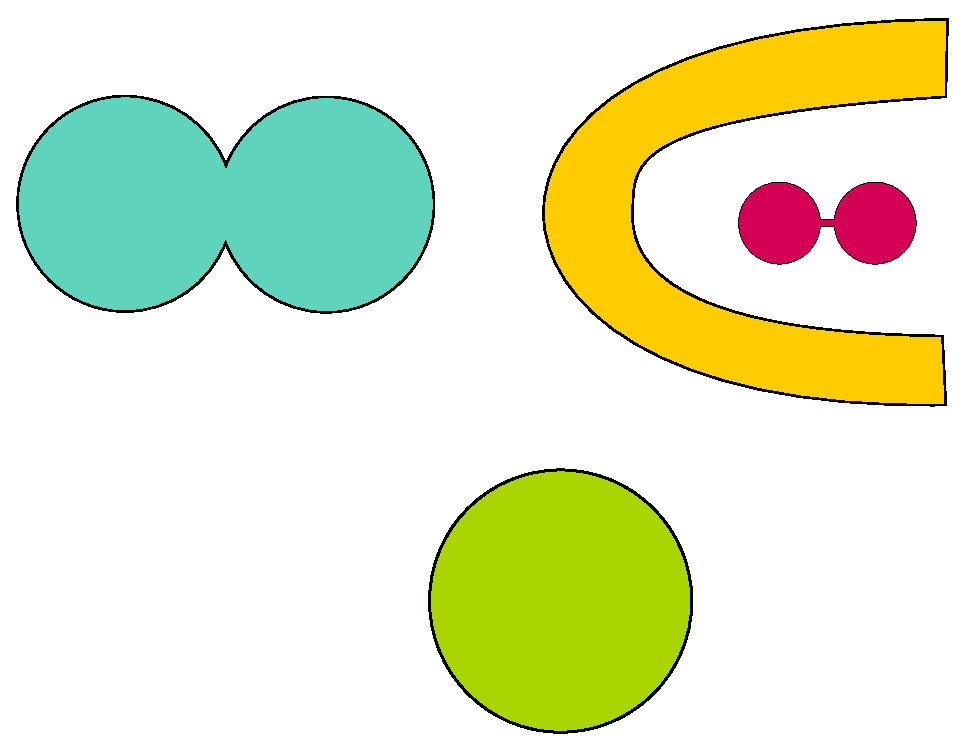
\includegraphics[width=.5\linewidth]{img/contiguousClusters.eps}
  \caption{Souvislé shluky}
  \label{fig:contiguousClusters}
\end{subfigure}
\begin{subfigure}{.49\textwidth}
  \centering
  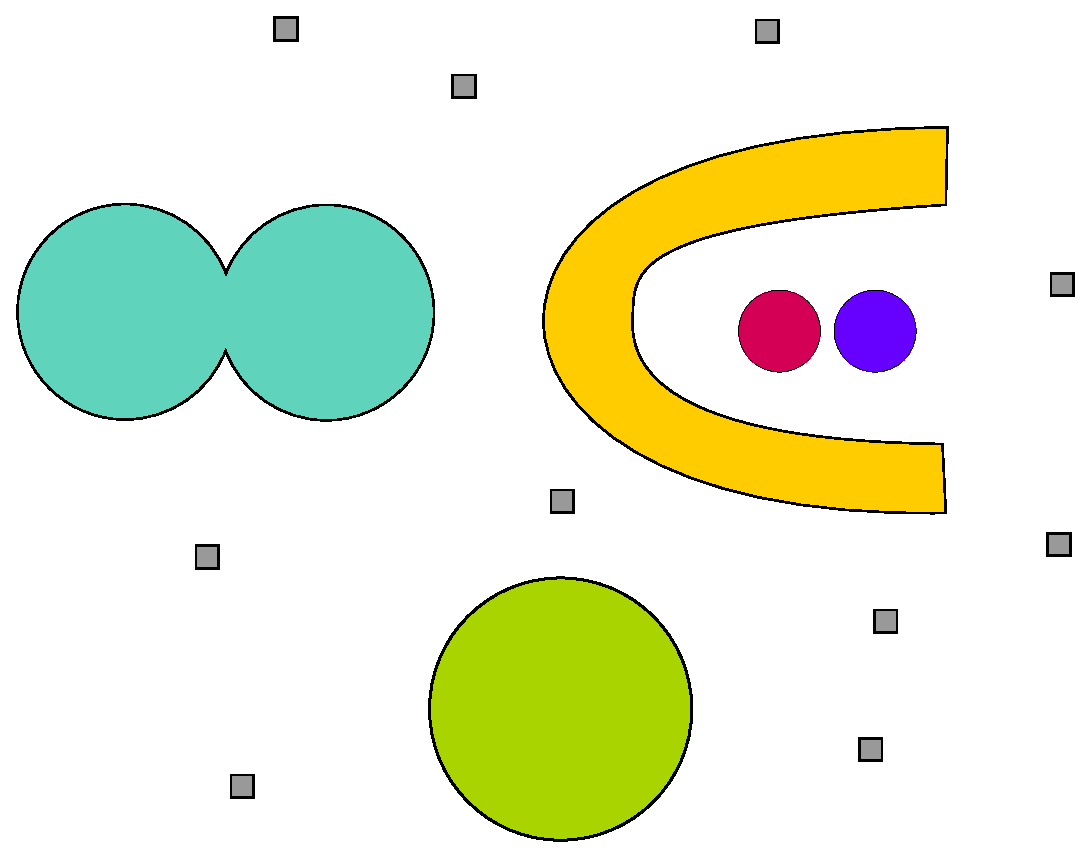
\includegraphics[width=.5\linewidth]{img/densityClusters.eps}
  \caption{Shluky založené na hustotě (šedé čtverečky představují šum)}
  \label{fig:densityClusters}
\end{subfigure}
\vspace*{0.5cm} 
\begin{subfigure}{.49\textwidth}
  \centering
  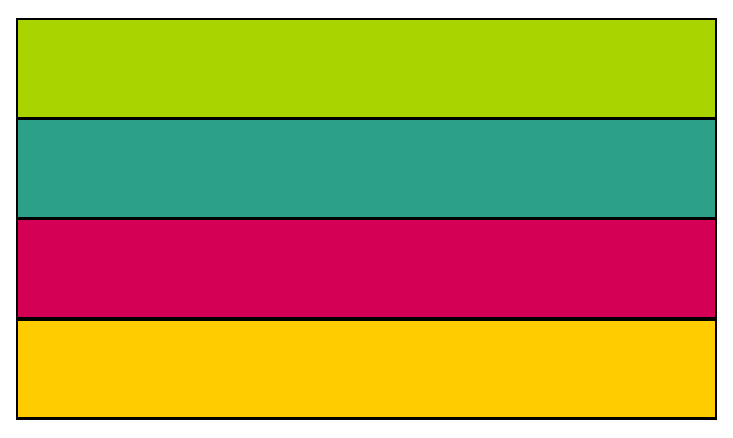
\includegraphics[width=.5\linewidth]{img/conceptualClusters.eps}
  \caption{Konceptuální shluky (Body ve shluku mají souřadnici y ze specifického rozsahu, ale souřadnice x se opomíjí)}
  \label{fig:conceptualClusters}
\end{subfigure}
\begin{subfigure}{.49\textwidth}
  \centering
  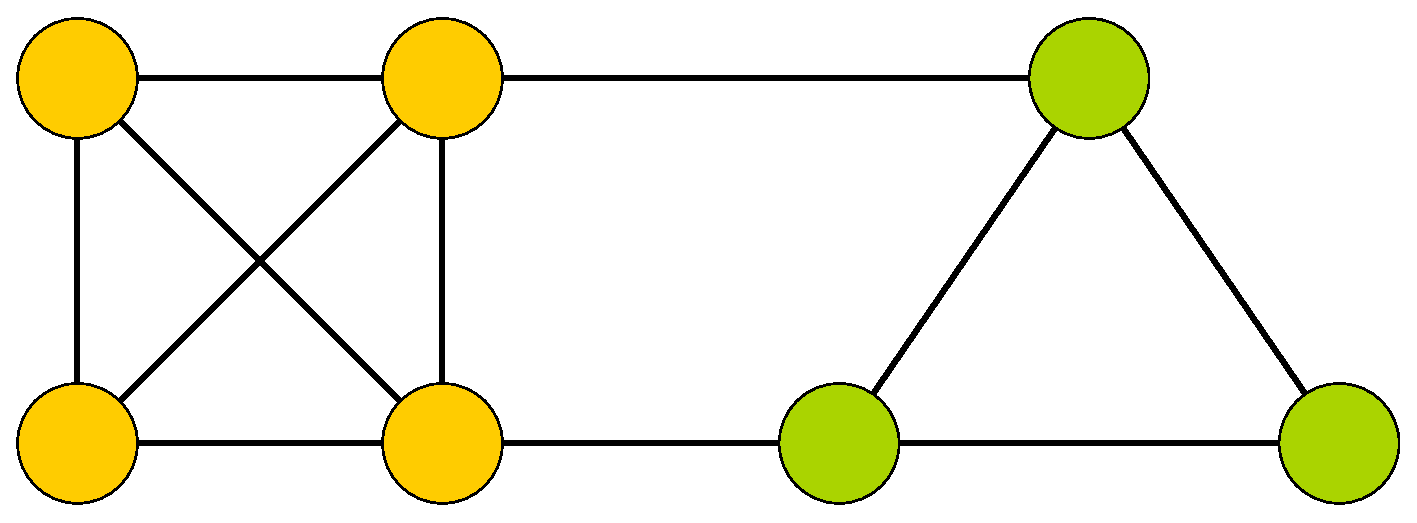
\includegraphics[width=.5\linewidth]{img/graphClusters.eps}
  \caption{Grafově orientované shluky}
  \label{fig:graphClusters}
\end{subfigure}
\caption{Typické modely shluků}
\end{figure}

\begin{description}
\item[Dobře oddělené shluky] Objekty jsou snadno oddělitelné - části shluků se nepřekrývají a rozděluje je řídká nebo prázdná oblast. Shluk je sada objektů, takže každý objekt uvnitř shluku je bližší objektům z jeho shluku než objekty z jiných shluků~\autoref{fig:wellSeparatedObjects}. Jedná se o nejjednodušší vstup dat a většina algoritmů v tomto případě funguje dobře.

\item[Shluky založené na centroidech] Objekt patří do shluku, pokud je blíže centroidu vlastního shluku než centroidům z ostatních clusterů~\autoref{fig: centerBasedClusters}. Centroid je speciální objekt spočítaný předtím než se přiřazují objekty. Výsledek je podobný rozdělení prostoru do Voroného buněk. Shluky založené na centroidech jsou podobné právě Voroného buňkám z Voroného diagramu, kde jsou centroidy nazývány generátory. Tento model je vhodný pro algoritmy založené na vzdálenosti mezi objektem a centroidem.\\
Jedním z algoritmů pro řešení tohoto problému je \textit{\textbf {Shlukování na bázi centroidů}}, kde jsou centroidy brány jako generátory, který nemusí být součástí vstupní množiny. Toto shlukování je v podstatě optimalizačním problémem, kde hledáme centroidy tak, aby byla vzdálenost mezi body a centroidy nejnižší. Problémem je, že samotná optimalizace je NP-těžký problém a výsledek je pouze aproximací ideálního řešení. Aproximace se běžně provádí v mnoha iteracích, které sestávají z přiřazení shluků k objektům a počítání nových centroidů.

\item[Souvislé shluky] Tento model je podobný modelu shluků založených na centroidech, ale rozdíl je v tom, že pokud jsou sva shluky dostatečně blízko, mohou být spojeny do jednoho~\autoref{fig:contiguousClusters}. Jinými slovy, objekt patří do shluku, pokud je podobný jednomu nebo více objektům z daného shluku~\cite{Tan05}. \\
Hlavní myšlenka \textbf {souvislých shluků} je, že objekty, které jsou v okolí, jsou více příbuzné než objekty, které jsou dále. Tyto algoritmy tedy seskupují objekty pouze na základě jejich vzdálenosti. Každý shluk může být popsán součtem vzdáleností nebo maximální vzdáleností potřebnou pro připojení objektů ke shluku. Mají-li shluky tuto vlastnost, můžeme je hierarchicky uspořádat tak, že nadřazené shluky jsou jen málo vzdálené od objektů v nich obsažených. Tato hierarchie může být reprezentována jako dendrogram, což je stromový diagram zobrazující hierarchii shluků. Tato vlastnost může být použita jak pro hierarchické shlukování, tak pro pevné shlukování, pokud vynecháme hierarchii. \\
% This model is similar to Center-Based Clusters model but there is difference that two clusters could be merged into single one if they are close enough~\autoref{fig:contiguousClusters}. In other words, object is in cluster if it is similar to one ore more other objects from cluster~\cite{Tan05}.\\
%Main idea of \textbf{Contiguity-based clustering} is that objects that are nearby are more related than objects that are farther, so these algorithms grouping objects based on their distance only. Each cluster can be described by sum of distances or by maximum distance needed to connect objects in cluster. Having these cluster property, they can be easily ordered into hierarchy so parent clusters needs little more distance to connect its objects. This hierarchy could be represented as a dendrogram, which is tree diagram showing cluster hierarchy. Because this property, Contiguity-based clustering could be used for hierarchical clustering but also for hard clustering if we omit the hierarchy.\\

Propojení objektů uvnitř shluku může být problematické, protože shluk může obsahovat velké množství objektů a tak existuje mnoho možností, jak vypočítat vzdálenosti. Existuje několik metod pro výběr kritérií spojení mezi dvěma sadami objektů $A$ a $B$, $d$ je zvolená metrika:
%The connection of the objects inside cluster could be problematic. Simply, because cluster consists of many objects, there are many choices to compute the distance to. There are several methods for choosing linkage criteria between two sets of objects $A$ and $B$, $d$ is chosen metric:
\begin{description}
\item[Maximální nebo úplná vazba shluků] $$\max\{d(a,b) : a \in A, b \in B\}$$
\item[Minimální nebo jedinečná vazba shluků] $$\min\{d(a,b) : a \in A, b \in B\}$$
\item[Průměr, průměrná shluková vazba nebo UPGMA] (Unweighted Pair Group Method with Arithmetic Mean) $$\frac{1}{|A||B|}\sum_{a \in A} \sum_{b \in B} d(a,b)$$
\item[centroidová vazba shluků nebo UPGMC] (Unweighted Pair-Group Method using Centroids) $$\|c_a - c_b\| \mbox{ kde } c_a \mbox{ and } c_b \mbox{ jsou centroidy shluků } A \mbox{ and } B$$
Toto může vypadat jako shlukování založené na centroidech, ale jde pouze o kritérium vazby a výsledkem jsou hierarchicky uspořádané shluky.
\item[Minimální shluková energie] $$\frac{2}{|A||B|}\sum_{i,j=1}^{|A|,|B|}\|a_i-b_j\|_2-\frac{1}{n^2}\sum_{i,j=1}^{|A|}\|a_i-a_j\|_2-\frac{1}{|B|^2}\sum_{i,j=1}^{m}\|b_{i}-b_{j}\|_{2} : a \in A, b \in B$$
\end{description}

Tyto metody nejsou odolné proti extrémním objektům, které způsobují vytváření nových shluků nebo dokonce sloučení jiných. Metody mají obecně složitost $O(n^3) $, takže pro velké množství dat jsou pomalé. Pro speciální případy existují optimalizace, které mají jen složitost $O(n^2) $. Tyto metody jsou však považovány za zastaralé.
%These methods are not resistive for extreme objects, which cause generating new clusters or even merging others. Methods has generally $O(n^3)$ complexity so they are slow for large amount of data. There exist optimization for special cases which has only complexity $O(n^2)$. These methods are taken as obsolete.

\item[Shluky založené na hustotě] Shluky jsou husté oblasti objektů oddělené oblastmi s nízkou hustotou. Tato metoda je vhodná pro případy, kdy vstupní data obsahují šum, protože oblasti s nízkou hustotou je odfiltrují a seskupení se nezmění.~\autoref{fig:densityClusters} \\
Shluky v založené na hustotě jsou definovány jako oblasti s vyšší hustotou objektů než ve zbývajících vstupních datech. Samostatné objekty jsou brány jako šum. Jedna z nejpopulárnějších metod je \textit{DBSCAN}. Jde o podobnou metodu jako souvislé shlukování, protože spojuje body na základě vzdálenosti, ale s rozdílem, že spojuje pouze body splňující kritérium hustoty. To znamená, že v okolí určeném vzdáleností musí být alespoň minimální počet objektů. Tyto objekty se pa nazývají jádro a vytváří základ shluku. Objekty, které nesplňují kritérium hustoty, ale jsou dostatečně blízko k alespoň jednomu bodu ze shluku, se přidávají do shluku. \\
Výhodou této metody je její výpočetní nenáročnost, protože vyžaduje pouze lineárně dotazů na rozsah. Tato metoda je navíc deterministická, takže ji není potřeba spouštět v iteracích.
Nevýhodou této metody je parametr hustoty $\epsilon$, protože při špatném nastavení mohou být hranice shluků s menší hustotou interpretovány jako šum. Problémy způsobují taky shluky, které leží blízko sebe, protože mohou být chápány jako jeden.

%Clusters are dense regions of objects. They are separated by low-density regions. This method is useful when some noise is present because the low-density regions will cover them and clusters will not change.~\autoref{fig:densityClusters} \\
%Clusters in \textbf{Density-based clustering} are defined as areas with higher density of objects than in the rest of input data. Standalone objects are taken as noise. One of the most popular method is \textit{DBSCAN}. It is similar to contiguity-based clustering, because it connecting points based on the distance, but it only connects %points satisfying density criterion. This means that in neighborhood specified by distance must be a minimum number of objects. These objects are called core objects and form the basis of cluster. Than objects which do not satisfy the density criterion but are close enough to at least one point from the cluster are added to cluster too.\\
%The advantage of this method is its computational unpretentiousness, because it require only linear number of range queries. This method is deterministic so there is no need to run it in iterations.
%Drawback of these methods is the $\epsilon$ density parameter so borders of clusters with smaller density could be interpreted as  noise. Also separating nearby clusters may cause problems to these methods.

\item[Distribuční modely shluků] Shluky v distribučních modelech jsou objekty, které patří ke stejné distribuci pravděpodobnosti. Model umožňuje, aby jeden objekt patřil do více shluků. \\
V tomto modelu jsou shluky definovány jako objekty ze stejné nebo podobné distribuce. Tento přístup v podstatě napodobuje proces generování vstupních dat a snaží se rekonstruovat ztracené statistické parametry. Hlavní problém tohoto modelu shluků je problém známý jako \textit{overfitting}, což znamená, že komplexnější model je popsán méně složitým a rozdíl mezi nimi je označen jako odchylka nebo šum. Například 3 body z okolí vrcholu paraboly budou popsány lineární funkcí. \\
Jednou z metod používaných v distribučním shlukování je \textit {Gaussian mixture models}, kde algoritmus iterativně optimalizuje parametry pevného počtu Gaussových distribucí.
Tato metoda předpokládá vstupní množinu s daty odpovídajícími Gaussově distribuci, ale problémem je, že data nemusí mít vůbec žádný model.

\item[Konceptuální shluky] Objekty uvnitř shluku mají některé vlastnosti stejné nebo podobné, ale jiné vlastnosti se mohou významně lišit.~\autoref{fig:conceptualClusters} \\
Jako algoritmus pro konceptuální shluky můžeme použít algoritmus, který závisí na jiných vlastnostech modelu a méně významné vlastnosti objektů lze snadno odfiltrovat.

\item[Grafově orientované shluky] Shluky mohou být definovány například jako kliky v grafech. Klika je podmnožina uzlů, kde je každý uzel spojen hranou s ostatními v klice.~\autoref{fig:graphClusters} \\
Kvůli speciálním požadavkům tohoto modelu jsou zapotřebí speciální algoritmy. Musíme tedy použít konkrétní grafové algoritmy jako je například algoritmus Bron-Kerbosch ~\cite{Sun15} pro nalezení klik.
\end{description}

\subsection{K-Means} 
Shlukovací algoritmy jsou širokou třídou algoritmů. Nemohli jsme se tedy soustředit na všechny modely, jejichž algoritmy bychom urychlovali paralelizací, protože k ejjich urychlení neexistuje žádný univerzální přístup. Pokud chceme urychlit algoritmus co nejefektivněji, musíme naopak využít každý detail konkrétního algoritmu. Potřebujeme tedy zvolit jeden z nejvšestrannějších algoritmů, na který se následně zaměříme. Jako vhodného reprezentanta jsme se zvolili algoritmus k-means kvůli jeho široké škále využití a nezávislosti na vlastnostech vstupních dat. \\
K-means algoritmus~\cite{Aggarwal13, Tan05} je algoritmus využívající shlukový modelu založený na centroidech. Vstupem je K-menas je množina $n$ bodů v $d$-dimenzionálním prostoru $R^d$, počet výstupních shluků $k$ a volitelném počtu iterací $ i $. \\
Úkolem je přidělit body centroidům (středům shluků) a minimalizovat vzdálenost mezi centroidem shluku a body obsaženými v tomuto shluku. Algoritmus funguje iterativně a každá iterace se skládá ze dvou kroků. V prvním kroku je pro každý bod nalezen nejbližší centroid a tento bod je přidělen do shluku, který k centroidu náleží. Ve druhém kroku jsou nové centroidy vypočítány jako průměr všech bodů přidělených stejnému shluku. Algoritmus končí po předem daném počtu kroků nebo když se mezi dvěma iteracemi nic nezmění. \\
Výstupem tohoto algoritmu jsou souřadnice centroidů a body s přiřazenými shluky.

%Clustering algorithms are wide class of algorithms and we could not focused on every clustering model and appropriate algorithm and speed it up by parallelization, because there does not exist any universal approach for speeding up but on the contrary it needs to use every single detail of the algorithm. We want to choose one of the most versatile algorithm so we decided for k-means algorithm for its wide range of usage and undemanding on the properties of the input data.\\
%K-means algorithm~\cite{Aggarwal13,Tan05} is centroid based clustering algorithm. K-means input is set of $n$ points in $d$-dimensional space $R^d$, a number of output clusters $k$ and a optional number of maximum iterations $i$. \\
%The task is to assign points to centroids (centers of clusters) and minimize the distance between cluster's centroid and points assigned to this cluster. Algorithm works iteratively and each iteration consist of two steps. At first step the nearest centroid is found for each point and this point is assigned to centroid's cluster. In the second step, new centroids are computed as a mean of all points assigned to same cluster. Algorithm ends after known number of steps or when nothing changes between two iterations.\\
%Output of the this algorithm are centroids coordinates and points with assigned clusters.


\algdef{SE}[REPEAT]{Repat}{Until}{\algorithmicrepeat}[1]{\algorithmicuntil\ #1}

\begin{algorithm}
\caption{K-means}\label{alg:kmeans}
\begin{algorithmic}[1]
\State Vyber K bodů jako iniciální centroidy
\Repeat
\State Vytvoř K shluků přiřazením bodů k nejbližším centroidům
\State Aktualizuj centroidy
\Until{centroidy se nezměnily nebo bylo dosaženo maximálního počtu iterací}
\end{algorithmic}
\end{algorithm}

Protože v prvním kroku neznáme centroidy, často se jako počáteční hodnoty používá prvních $k$ bodů vstupní množiny. Algoritmus K-means konverguje rychle během několika prvních iterací, takže podmínku zastavení můžeme pozměnit na "Změnilo se jen relativně málo centroidů". \cite{Tan05}. \\
Složitost výpočtu je $O(n*k*i*d)$, kde $n$ je počet vstupních bodů, $k$ je počet clusterů, $i$ je počet iterací a $d$ je dimenze vstupních dat. \\

Abychom mohli vyhodnotit výstup k-means, musíme uměnit měřit kvalitu přiřazení do klastrů. Pro tento účel se nejčastěji používá funkce \textbf{Sum of Squared Error (SSE)}. Chyba jednoho bodu je reprezentována vzdáleností od centroidu daného shluku a SSE funkce sčítá čtverce chyb jednotlivých bodů.
$$SSE = \sum^k_{i=1}\sum_{o \in O_i}|o,c_i|^2, \textrm{ $c_i$ \textit{je středem shluku} $O_i$ }$$
Pokud dostáváme výsledky se špatným $SSE$, můžeme jej snížit například zvýšením počtu klastrů $k$, ale pokud jsou počáteční klastry vybrány špatně, nemusí to pomoci.

Počáteční centroidy jsou jednou z nevýhod k-means algoritmu, protože jejich počet potřebujeme znát již na začátku a po počátečním výpočtu toto číslo už nelze změnit. Tuto možnost mohou ale některé typy problémů vyžadovat a tak jsou pro ně k-means nepoužitelné. Dalším problémem je výběr počátečních centroidů. Ačkoliv zvolíme ideální $k$ pro vstupní data, pravděpodobnost, že jsme zvolili objekty z různých klastrů jako počáteční centroidy, je opravdu malá~\cite{Tan05}: $$P = \frac{\mbox{počet způsobů jakým můžeme vybrat jeden bod z každého shluku}}{\mbox{počet možností jakými můžeme zvolit K centroidů}}=\frac{k!{n \choose k}}{k^k {n \choose k} }=\frac{k!}{k^k}$$ Tato pravděpodobnost se blíží nule i pro relativně malé $k$. Například pro $k=10$, je pravděpodobnost $0.00036$. \\
Existují ale způsoby, jak tento problém vyřešit a vybrat lepší počáteční body~\cite{Tan05}:
\begin{description}
\item[více běhů] k-means je spuštěn několikrát s různými počátečními body a jako výstup je vybrán nejlepší výsledek.
\item[vzorkování] Počáteční cenroidy jsou vybrány na základě ovzorkování vstupních dat hierarchicjým shlukování.
\item[více centroidů] Je vybráno více centroidů než je vstupní $k$ a z nich se vyberou ty nejlépe rozmístěné.
\item[následné zpracování] Výsledek algoritmu je následné zpracován - Shluky s nejvyšším $SSE$ jsou rozděleny a na druhou stranu shluky s nejnižším $SSE$ mohou být spojeny.
\end{description} 

Dalším problémem k-means je, že základní verze může produkovat prázdné shluky. To lze vyřešit aktualizací algoritmu: pokud najdeme prázdný shluk, můžeme ho nahradit bodem, který nejvíce přispívá k $SSE$. Další možností je vybrat bod z clusteru s největším $SSE$ ~\cite{Tan05}.

Pokud se shluky výrazně liší v rozměrech/hustotě nebo jde-li o nekulovité útvary, má pak shluková analýza problém s nalezením prostředků shluků~\cite{Tan05}. \\
Jelikož je hlavním cílem k-means nalézt shluky s podobnou velikostí, budeme mít problém se vstupními daty, které obsahují jeden velký shluk s mnoha objekty a jeden menší shluk s několika málo objekty~\autoref{fig:kmeansbadinputsize}. k-means potom rozdělí větší shluk~\autoref{fig:kmeansbadoutputsize}, takže objekty, které náleží logicky do většího shluku, ale zároveň jsou blíže centroidu z menšímu shluku, jsou přiřazeny k menšímu shluku, což může být nežádoucí. Je to dáno tím, že k-means ignorují distribuci vstupních dat.

\begin{figure}[h]
\centering
\begin{subfigure}{.49\textwidth}
  \centering
  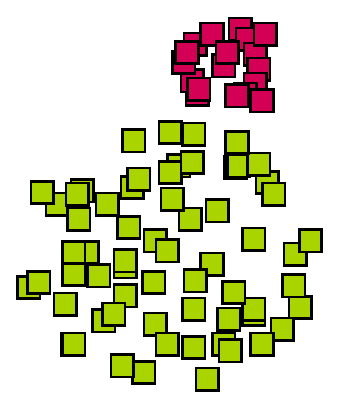
\includegraphics[width=.5\linewidth]{img/kmeans_badInputSampleSize.eps}
  \caption{Vstupní data (rozřazené do shluků jen pro ilustraci)}
  \label{fig:kmeansbadinputsize}
\end{subfigure}
\begin{subfigure}{.49\textwidth}
  \centering
  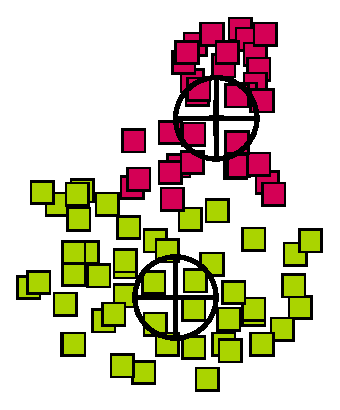
\includegraphics[width=.5\linewidth]{img/kmeans_badOutputSampleSize.eps}
  \caption{výstup k-means}
  \label{fig:kmeansbadoutputsize}
\end{subfigure}
\caption{K-means nad shluky různých velikostí}
\end{figure}

Také hustota shluků může způsobovat k-means problémy. Když máme dva husté shluky blízko sebe a jeden vzdálenější shluk s nízkou hustotou~\autoref{fig:kmeansbadinputdensity}, k-means obvykle označují husté shluky jako jeden a rozdělí řídký shluk do více shluků.~\autoref{fig:kmeansbadoutputdensity}
\begin{figure}[h]
\begin{subfigure}{.49\textwidth}
  \centering
  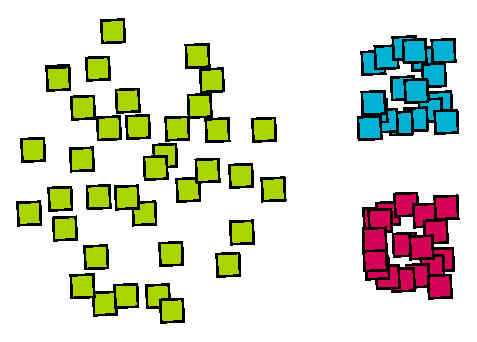
\includegraphics[width=.5\linewidth]{img/kmeans_badInputSampleDensity.eps}
  \caption{Vstupní data (rozřazené do shluků jen pro ilustraci)}
  \label{fig:kmeansbadinputdensity}
\end{subfigure}
\begin{subfigure}{.49\textwidth}
  \centering
  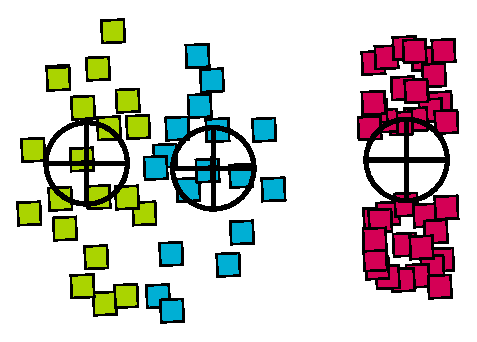
\includegraphics[width=.5\linewidth]{img/kmeans_badOutputSampleDensity.eps}
  \caption{výstup k-means}
  \label{fig:kmeansbadoutputdensity}
\end{subfigure}
\caption{K-means nad shluky různé hustoty}
\end{figure}

Dalším problémem je, že k-means algoritmus nerozpozná tvar shluku a produkuje pouze kulové shluky. To je problém, pokud dva obvykle nekonvexní shluky~\autoref{fig:kmeansbadinputshape} jsou dostatečně blízko a jeden zasahuje do konvexního obalu toho druhého.K-means pak obvykle přidělují body z jednoho shluku do druhého a naopak~\autoref{fig:kmeansbadoutputshape}.
\begin{figure}[h]
\begin{subfigure}{.49\textwidth}
  \centering
  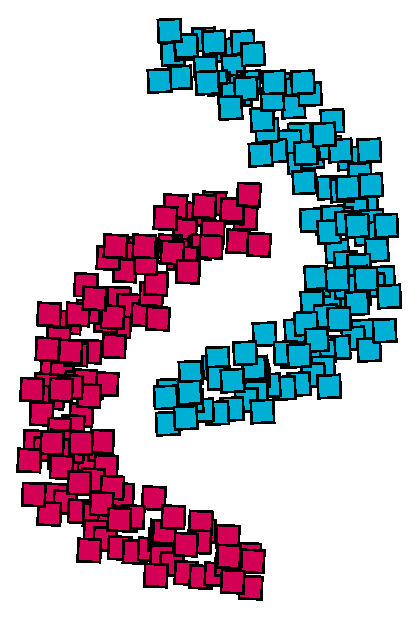
\includegraphics[width=.5\linewidth]{img/kmeans_badInputSampleShape.eps}
  \caption{Vstupní data (rozřazené do shluků jen pro ilustraci)}
  \label{fig:kmeansbadinputshape}
\end{subfigure}
\begin{subfigure}{.49\textwidth}
  \centering
  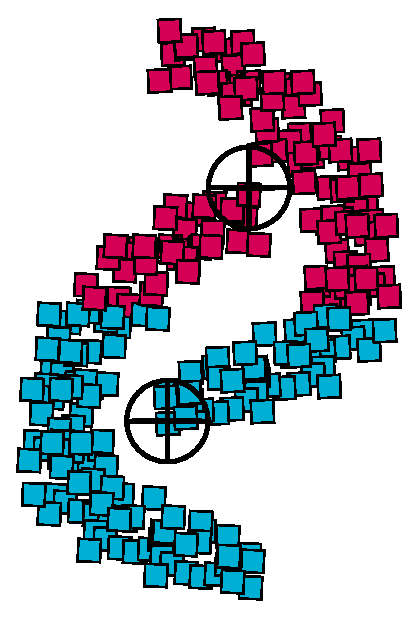
\includegraphics[width=.5\linewidth]{img/kmeans_badOutputSampleShape.eps}
  \caption{výstup k-means}
  \label{fig:kmeansbadoutputshape}
\end{subfigure}
\caption{K-means nad nekulovitými shluky}
\end{figure}

Tyto problémy mohou být vyřešeny použitím více shluků, než přirozeně vyžadují vstupní data. Například vstupní data~\autoref{fig:kmeansbadinputshape} obsahují dva přirozené shluky, ale když se pokusíme rozdělit data na více shluků, výsledek bude obsahovat malé shluky, které obsahují body z jednoho přirozeného shluku a neobsahují shluky z druhého~\autoref{fig:kmeansbadoutputsolution}. Pokud tyto informace následně zpracujeme, můžeme získat očekávaný výsledek a zabránit tomuto nedostatku k-means.
\begin{figure}[h]
  \centering
  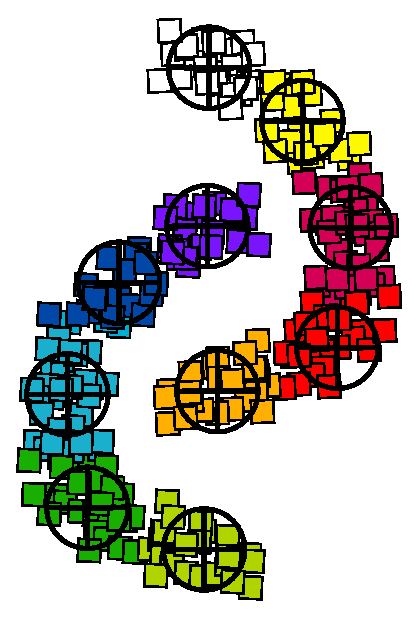
\includegraphics[width=.3\textwidth]{img/kmeans_badOutputSampleShapeSolution.eps}
  \caption{řešení k-means pro shluky špatných tvarů}
  \label{fig:kmeansbadoutputsolution}
\end{figure}


\subsubsection{Varianty k-means}
Protože k-means jsou univerzálním algoritmem, existují různé varianty pro případy, kdy je klasický algoritmus k-prostředků nevhodný nebo nepoužitelný. Tyto varianty mohou vyřešit některé problémy a omezení klasického algoritmu k-means.
\begin{description}
\item[k-medoids] - centroidy nejsou uměle vytvořené body v prostoru $R^d$, ale reálné body ze vstupních dat, jejichž průměrná odchylka od ostatních bodů ve shluku je minimální (místo průměru se využívá medián).
\item[k-medians] - stejný algoritmus jako k-means, ale pro výpočet nového centroidu se v každé dimenzi využívá medián místo výpočtu průměrné hodnoty.
\item[k-means++] - Počáteční centroidy jsou vybrány náhodně. Tím lze zabránit potenciálním špatným vstupům.
\item[Fuzzy C-means] - jsou povoůeny neostré shluky~\ref{sec:clusterorganization}. Objekty nepatří striktně jednomu shluku, ale uvažujeme stupeň náležení k jednotlivých shlukům. Pro výpočet nových centroidů se využívá vážený průměr (kde je jako váha brán stupeň náležení).
\item[Rozdělující (Bisecting) k-means]~\cite{Tan05} je varianta k-means, která produkuje hierarchické uspořádání shluků.Pracuje, stejně jako k-means, iterativně, ale v každém kroku je shluk s nejvyšším $SSE$ rozdělen na 2 pomocí klasického k.means algoritmu s parametrem $k=2$. Algoritmus iteruje, dokud nedosáhne daného počtu shluků.~\autoref{alg:bisectingkmeans}
\begin{algorithm}
\caption{Rozdělující k-means}\label{alg:bisectingkmeans}
\begin{algorithmic}[1]
\State Vlož všechny body do seznamu shluků jako jeden shluk-
\Repeat
\State Vyber první shluk ze seznamu shluků
\For{i=1 do daného počtu iterací}
\State Rozděl vybraný shluk pomocí základního k-means algoritmu
\EndFor
\State Přidej dva shluky vzniklé rozdělením s nejnižším SSE do seznamu shluků
\State Aktualizuj centroidy pro každá shluk
\Until{seznam shluků obsahuje k shluků}
\end{algorithmic}
\end{algorithm}

\end{description}
